\NeedsTeXFormat{LaTeX2e}

% The following saves the original definitions of \geq and \leq (guide only).
\let\realgeq\geq
\let\realleq\leq

\documentclass{fac}

\ifprodtf \else \usepackage{latexsym}\fi

% The following macros automatically define symbols to be used in Table 1 of
% the authors' guide, using characters from the AMS symbol font MSAM.

\newcommand\black{\ensuremath{\blacktriangleright}}
\newcommand\white{\ensuremath{\vartriangleright}}

\newif\ifamsfontsloaded
\ifprodtf
  \newcommand\whbl{\white\kern-.1em--\kern-.1em\black}
  \newcommand\blwh{\black\kern-.1em--\kern-.1em\white}
  \newcommand\blbl{\black\kern-.1em--\kern-.1em\black}
  \newcommand\whwh{\white\kern-.1em--\kern-.1em\white}
  \amsfontsloadedtrue
\else
  \checkfont{msam10}
  \iffontfound
    \IfFileExists{amssymb.sty}
      {\usepackage{amssymb}\amsfontsloadedtrue
       \newcommand\whbl{\white\kern-.125em--\kern-.125em\black}%
       \newcommand\blwh{\black\kern-.125em--\kern-.125em\white}%
       \newcommand\blbl{\black\kern-.125em--\kern-.125em\black}%
       \newcommand\whwh{\white\kern-.125em--\kern-.125em\white}}
      {}
  \fi
\fi

%% Macros for the guide only %%
\newcommand\eg{\textit{e.g.\ }}
\newcommand\ie{\textit{i.e.\ }}
\newcommand\etc{\textit{etc}}
\newcommand\hatp{\skew3\hat{p}}
\newcommand\lra{\ensuremath{\quad\longrightarrow\quad}}
\providecommand\AMSLaTeX{AMS\,\LaTeX}
%% End of macros for the guide %%

\newtheorem{theorem}{Theorem}[section]

\title{A Relational Static Semantics for\\
		\ Call Graph Construction}

\author[Xilong Zhuo and Chenyi Zhang]
    {Xilong Zhuo$^1$ and Chenyi Zhang$^2$\\
     $^1$College of Information Science and Technology, Jinan University, Guangzhou, China\\
     $^2$College of Information Science and Technology, Jinan University, Guangzhou, China}

\correspond{Chenyi Zhang.
            e-mail: chenyi\_zhang@jnu.edu.cn}

%\pubyear{2000}
\pagerange{\pageref{firstpage}--\pageref{lastpage}}

\newtheorem{Definition}{Definition}
\newtheorem{Theorem}{Theorem}
\newtheorem{Lemma}{Lemma}
\newtheorem{Property}{Property}
\newtheorem{Corollary}{Corollary}
\newtheorem{Proof}{Proof}

\newcommand{\keyword}[1]{\mathsf{#1}}
\newcommand{\kw}[1]{\keyword{#1}}

\newcommand{\kwnull}[0]{\keyword{null}}
\newcommand{\kwnew}[0]{\keyword{new}}
\newcommand{\kwextends}[0]{\keyword{extends}}
\newcommand{\kwclass}[0]{\keyword{class}}
\newcommand{\kwthis}[0]{\keyword{this}}
\newcommand{\kwif}[0]{\keyword{if}}
\newcommand{\kwthen}[0]{\keyword{then}}
\newcommand{\kwelse}[0]{\keyword{else}}
\newcommand{\kwskip}[0]{\keyword{skip}}

\newcommand\Var{\mathtt{VAR}}
\newcommand\Val{\mathtt{V}}
\newcommand\Obj{\mathtt{OBJ}}

\newcommand{\VPT}{\Omega}
\newcommand{\HPT}{\Phi}
\newcommand{\Class}{\mathcal{C}}
\newcommand{\Field}{\mathcal{F}}
\newcommand{\bigO}{\mathcal{O}}
\newcommand{\word}[1]{\langle #1\rangle}
\newcommand{\Nat}{\mathbb{N}}
\newcommand{\less}{\sqsubseteq}
\newcommand{\tflow}{\dashrightarrow}
\newcommand{\hflow}{\longrightarrow}
\newcommand{\lhflow}[1]{\stackrel{#1}{\hflow}}
\newcommand{\lhflowstar}[1]{\stackrel{#1}{\longrightarrow^*}}

\newcommand\Loc{\mathcal{L}}
\newcommand\Label{\Phi}
\newcommand\set[1]{\{#1\}}
\newcommand\power{\mathcal{P}}
\newcommand\join{\cup}
\newcommand\subtype{\subseteq}

\usepackage{amsfonts}
\usepackage{amsmath}
\usepackage{amssymb}
\usepackage{threeparttable}
\usepackage{graphicx}
\usepackage{color}
\usepackage{verbatimbox}
\usepackage{url}
\usepackage{subfigure}

\definecolor{lbcolor}{rgb}{1,1,1}

\usepackage{listings}
\lstset{
  backgroundcolor=\color{lbcolor},
  language=java,
  frame=single,
  numbers=left,
  stepnumber=1,    
  firstnumber=1,
  numberfirstline=true,
  tabsize=4,
  captionpos=b,
  keywordstyle=\color[rgb]{0,0,1},
  commentstyle=\color[rgb]{0.133,0.545,0.133},
  stringstyle=\color[rgb]{0.627,0.126,0.941}
}

\begin{document}
\label{firstpage}

\makecorrespond

\maketitle

\begin{abstract}
The problem of resolving virtual method and interface calls in object-oriented languages has been a long standing challenge to the program analysis community. The complexities are due to various reasons, such as increased levels of class inheritance and polymorphism in large programs. In this paper, we propose a new approach called type flow analysis that represent propagation of type information between program variables by a group of relations without the help of a heap abstraction. We prove that regarding the precision on reachability of class information to a variable, our method produces results equivalent to that one can derive from a points-to analysis.
Moreover, we implement a static type analysis tool for our approach. To evaluate our method, we use instrumentation tenichque to implement a dynamic profilling type recorder. The experimental results show that our approach is more practical in both efficency and accuracy.
\end{abstract}

\begin{keywords}
Type Analysis; Static Analysis; Method Resolving; Call Graph
\end{keywords}

\section{Introduction}\label{sec:introduction}
For object-oriented programming languages, virtual methods (or functions) are those declared in a base class but are meant to be overridden in different child classes. Statically determine a set of methods that may be invoked at a call site is important to program optimization, from results of which a subsequent optimization may reduce the cost of virtual function calls or perform method inlining if target method forms a singleton set, and one may also remove methods that are never called by any call sites, or produce a call graph which can be useful in other optimization~processes.

Efficient solutions, such as Class Hierarchy Analysis (CHA)~\cite{Dean1995,Fernandez1995}, Rapid Type Analysis (RTA)~\cite{Bacon1996} and Variable Type Analysis (VTA)~\cite{Sundaresan2000}, conservatively assign each variable a set of class definitions, with relatively low precision. Alternatively, with the help of an abstract heap, one may take advantage of points-to analysis~\cite{andersen94} to compute a set of object abstractions that a variable may refer to, and resolve the receiver classes in order to find associated methods at call sites.

The algorithms used by CHA, RTA and VTA are conservative, which aim to provide an efficient way to resolve calling edges, and which usually take linear-time in the size of a program, by focusing on the types that are collected at the receiver of a call site. For instance, let $x$ be a variable of declared class $A$, then at a call site $x.m()$, CHA will draw a call edge from this call site to method $m()$ of class $A$ and every definition $m()$ of a class that extends $A$. In case class $A$ does not define $m()$, a call edge to an ancestor class that defines $m()$ will also be included. For a variable $x$ of declared interface $I$, CHA will draw a call edge from this call site to every method of name $m()$ defined in class $X$ that implements $I$.
We write $CHA(x,m)$ for the set of methods that are connected from call site $x.m()$ as resolved by  Class Hierarchy Analysis (CHA).
Rapid Type Analysis (RTA) is an improvement from CHA which resolves call site $x.m()$ to $CHA(x,m)\cap inst(P)$, where $inst(P)$ stands for the set of methods of classes that are instantiated in the program.

\begin{figure}
\begin{minipage}[t]{0.5\linewidth}
\centering
\begin{verbbox}
class A{
    A f;
    void m(){
        return this.f;
    }
}

class B extends A{}

class C extends A{}
\end{verbbox}
\theverbbox
\end{minipage}
\begin{minipage}[t]{0.5\linewidth}
%\center
\centering
\begin{verbbox}
1:  A x = new A();  //O_1
2:  B b = new B();  //O_2
3:  A y = new A();  //O_3
4:  C c = new C();  //O_4
5:  x.f = b;
6:  y.f = c;
7:  z = x.m();
\end{verbbox}
\theverbbox
\end{minipage}
\caption{An example that compares precision on type flow in a program.}\label{figure:example}
\end{figure}

Variable Type Analysis (VTA) is a further improvement. VTA defines a node for each variable, method, method parameter and field. Class names are treated as values and propagation of such values between variables work in the way of value flow.
As shown in Figure~\ref{figure:vta} (example code in figure~\ref{figure:example}), the statements on line $1-4$ initialize type information for variables $x$, $y$, $b$ and $c$,
and statements on line $5-7$ establish value flow relations. Since both $x$ and $y$ are assigned type $A$, $x.f$ and $y.f$ are both represented by node $A.f$, thus the set of types reaching $A.f$ is now $\set{B,C}$. (Note this is a more precise result than CHA and RTA which assign $A.f$ with the set $\set{A,B,C}$.)
Since $A.m.this$ refers to $x$, $this.f$ inside method $A.m()$ now refers to $A.f$. Therefore, through $A.m.return$, $z$ receives  $\set{B,C}$ as its final set of reaching types.

\begin{figure}%%[ht]
\begin{tabular}{cc}

\begin{minipage}[h]{0.5\linewidth}
\centering
\begin{tabular}{|c|c|}
  \hline
  \textbf{Statement} & \textbf{VTA fact} \\
   \hline
  \hline
  % after \\: \hline or \cline{col1-col2} \cline{col3-col4} ...
  $A\ x = \kwnew\ A()$ & $x\leftarrow A$ \\ \hline
  $B\ b = \kwnew\ B()$ & $b\leftarrow B$ \\ \hline
  $A\ y = \kwnew\ A()$ & $y\leftarrow A$ \\ \hline
  $C\ c = \kwnew\ C()$ & $c\leftarrow C$ \\ \hline
  $x.f = b$ & $A.f\leftarrow b$ \\ \hline
  $y.f = c$ & $A.f\leftarrow c$ \\ \hline
   & $A.m.this\leftarrow x$ \\
  $z = x.m()$  & $A.m.return\leftarrow A.f$ \\
   & $z\leftarrow A.m.return$\\
  \hline
\end{tabular}
\caption{VTA facts on the example}\label{figure:vta}
\end{minipage}
&
\begin{minipage}[h]{0.5\linewidth}
\centering
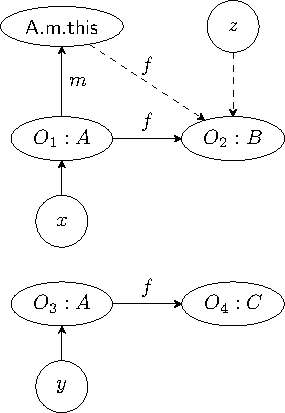
\includegraphics[width=3.5cm]{points-to.pdf}
\caption{Points-to results on the example}\label{figure:points-to}
\end{minipage}
\end{tabular}
\end{figure}

The result of a context-insensitive subset based points-to analysis~\cite{andersen94} creates a heap abstraction of four objects (shown on line $1-4$ of Figure~\ref{figure:example} as well as the ellipses in Figure~\ref{figure:points-to}). These abstract objects are then inter-connected via field store access defined on line $5-6$. The derived field access from $A.m.this$ to $O_2$ is shown in dashed arrow. By return of the method call $z=x.m()$, variable $z$ receives $O_2$ of type $B$ from $A.m.this.f$, which gives a more precise set of reaching types for variable $z$.

From this example, one may conclude that the imprecision of VTA in comparison with points-to analysis is due to the over abstraction of object types, such that $O_1$ and $O_3$, both of type $A$, are treated under the same type. Nevertheless, points-to analysis requires to construct a heap abstraction, which brings in extra information, especially when we are only interested in the set of reaching types of a variable.

\begin{figure}
\centering
%\vspace{5cm}
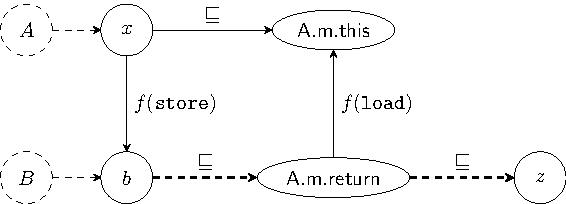
\includegraphics[width=8cm]{tfa.pdf}
\caption{Type Flow Analysis for variable $z$ in the example}\label{fig:tfa}
\end{figure}

In this paper we introduce a relational static semantics called Type Flow Analysis (TFA) on program variables and field accesses. Different from VTA, in addition to the binary value flow relation ``$\less$'' on the variable domain $\Var$, where $x\less y$ denotes all types that flow to $x$ also flow to $y$, we also build a ternary field store relation $\rightarrow\ \subseteq\Var\times\Field\times\Var$ to trace the \emph{load} and \emph{store} relationship between variables via field accesses. This provides us additional ways to extend the relations $\less$ as well as $\rightarrow$. %%For example given $x\lhflow{f}y$ and $x\less z$, we can derive $z\lhflow{f}y$.
%%
Taking the example from Figure~\ref{figure:example}, we are able to collect the store relation $x\lhflow{f}b$ from line $5$. Since $x\less \textsf{A.m.this}$, together with the implicit assignment which loads $f$ of $\textsf{A.m.return}$, we further derives $b\less\textsf{A.m.return}$ and $b\less z$ (dashed thick arrows in Figure~\ref{fig:tfa}). Therefore, we assign type $B$ to variable $z$. The complete reasoning pattern is depicted in Figure~\ref{fig:tfa}. Nevertheless, one cannot derive $c\less z$ in the same way.

%%% contributions with %%% discussion on context-sensitivity
We have proved that in the context-insensitive inter-procedural setting, TFA is as precise as the subset based points-to analysis regarding type related information. Since points-to analysis can be enhanced with various types of context-sensitivity on variables and objects (\eg, call-site-sensitivity~\cite{Shivers91,Kastrinis2013}, object-sensitivity~\cite{Milanova2005,Smaragdakis11,Tan16} and type-sensitivity~\cite{Smaragdakis11}), extending type flow analysis with context-sensitivity will only require to consider contexts on variables, which is left for future work.

We have implemented a static type analysis tool for context-insensitive type flow analysis, which is written in Java and aims to analyze Java programs. The implementation has been tested on a collection of benchmark programs from SPECjvm2008~\cite{specjvm}. We conducted several experiments to compare the efficency and accuracy with CHA and PTA implemented by Soot. In order to comparing accuracy, we used the instrument technique to implement a dynamic profilling tool, to extract the types of method receiver in runtime. We compared different static results with dynamic record. The experimental result has shown that our approach is more precise than CHA and as precise as PTA. Moreover, TFA reduce significant time cost than PTA. In addition, we found that both PTA and TFA do not provide soundness on all benchmarks. We detail looked into all the unmatch record to find out the reason for unsoundness, which involves some Java advanced features liked reflection, JNI, etc. We will discuss it in the experiment section of this paper. %(Need more citations here, and brief the experimental results.)

\section{Type Flow Analysis}\label{sec:type-flow-analysis}
We define a core calculus consisting of most of the key object-oriented language features, shown in Figure~\ref{fig:syntax}, which is designed in the same spirit as Featherweight Java~\cite{Igarashi2001}.
A program is defined as a code base $\overline{C}$ (i.e., a collection of class definitions) with statement $s$ to be evaluated.
To run a program, one may assume that $s$ is the default (static) entry method with local variable declarations $\overline{D}$,
similar to e.g., Java and C++, which may differ in specific language designs.
%% to consider dynamic semantics later: Let $S$ and $H$ be the runtime stack and heap, where $S:\Var\rightarrow \Val$maps local variables to values and $H:\Val\rightarrow \Obj\cup\set{\kwnull}$ maps values to objects.
We define a few auxiliary functions. Let function $fields$ maps class names to their fields, $methods$ maps class names to their defined or inherited methods, and $type$ provides types (or class names) for objects. Given class $c$, if $f\in fields(c)$, then $ftype(c,f)$ is the defined class type of field $f$ in $c$. Similarly, give an object $o$, if $f\in fields(type(o))$, then $o.f$ may refer to an object of type $ftype(type(o),f)$ or %%an object of
any of its subclass at runtime. Write $\Class$ for the set of classes, $\Obj$ for the set of objects, $\Field$ for the set of fields and $\Var$ for the set of variables that appear in a program.
\footnote{Sometimes we mix-use the terms \emph{type} and \emph{class} in this paper when it is clear from the context.}

\begin{figure}\centering
	\begin{tabular}[c]{lll}
		$C$&$::=$&$\kwclass\ c\ [\kwextends\ c] \ \{\overline{F};\ \overline{M}\}$\\
        $F$&$::=$&$c \ f$\\
        $D$&$::=$&$c \ z$\\
		$M$&$::=$&$m(x) \ \{\overline{D}; s; \kw{return}\ x'\}$\\
		$s$&$::=$&$e\mid x{=}\kwnew \ c\mid  x {=} e \mid x.f{=}y \mid s;s$\\

		$e$&$::=$&$ \kwnull\mid x \mid x.f \mid x.m(y) $\\
        $prog$&$::=$&$\overline{C};\overline{D}; s$\\
	\end{tabular}
	\caption{Abstract syntax for the core language. \label{fig:syntax}}
\end{figure}

In this simple language we do not model common types (\eg, int and float) that are irrelevant to our analysis. We focus on the reference types which form a class hierarchical structure. We assume a context insensitive setting, such that every variable can be uniquely determined by its name together with its enclosing class and methods.
For example, if a local variable $x$ is defined in method $m$ of class $c$, then $c.m.x$ is the unique representation of that variable. Therefore, it is safe to drop the enclosing class and method name if it is clear from the context.
In general, we have the following types of variables in our analysis: (1) local variables, (2) method parameters, (3) this reference of each method, all of which are syntactically bounded by their enclosing classes and methods.

We define three relation for catching type flow information in programs, a partial order on variables $\less\ \subseteq\Var\times\Var$, a type flow relation
$\tflow\subseteq\Class\times\Var$, as well as a field access relation $\hflow\subseteq\Var\times\Field\times\Var$,
which are initially given as follows.

\paragraph{Definition 1.}\label{def:base} (Base Relations)
These three basic relations represent program facts. They can be generated directly based on different statements syntactically appearing in programs.
\begin{enumerate}
  \item $c\tflow x$ if there is a statement $x = \kwnew\ c$;
  \item $y\less x$ if there is a statement $x = y $;
  \item $x\lhflow{f}y$ if there is a statement $x.f = y$.
\end{enumerate}
Intuitively, $c\tflow x$ means variable $x$ may have type $c$ (i.e., $c$ flows to $x$), $y\less x$ means all types flow to $y$ also flow to $x$, and $x\lhflow{f}y$ means that one may access variable $y$ from field $f$ together with variable $x$.\footnote{Note that VTA treats statement $x.f = y$ as follows. For each class $c$ that flows to $x$ which defines field $f$, VTA assigns all types that flow to $y$ also to $c.f$.}
We give a snippet code, as shown in Listing~\ref{lst:relation}, to illustrate the generation of relations. For statement ``$A\ a1\ =\ new A()$'' and ``$B\ b1\ =\ new B()$'', we generates two type flow relations, ''$A \tflow a1$'' and ``$B \tflow b1$'', respectively. Tow partial order relations, ``$a1 \less a2$'' and ``$a2 \less a3$'', are generated for the statements ``$a2\ =\ a1$'' and $a3\ =\ a2$. For the field store statement on line 6. We generate a field access relation ``$a1 \lhflow{f} b1$''. The final result is shown is Figure.~\ref{fig:basic-relation}, on which a dash circle refers to type and other nodes in gray background refer to variables. Type relation, partial order relation and field access relation are represented in dash arrow, arrow with label ``$\less$'' and arrow with label ``$f$'', respectively. 
\begin{lstlisting}[caption={Example for generation of relations},label={lst:relation}]
public void m() {
	A a1 = new A();
	a2 = a1;
	a3 = a2;
	B b1 = new B();
	a1.f = b1;
	b2 = a1.f;
	a4 = b2.m2(a3);
}

class B {
	public A m2(p1) {... return r;}
}
\end{lstlisting}
\begin{figure}
\centering
\subfigure[Basic relation for Listing~\ref{lst:relation}] {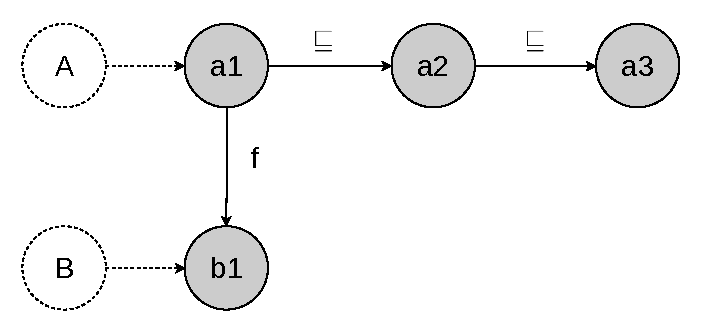
\includegraphics[scale=0.5]{basic-relation.pdf} \label{fig:basic-relation}}
\hspace{2cm}
\subfigure[] {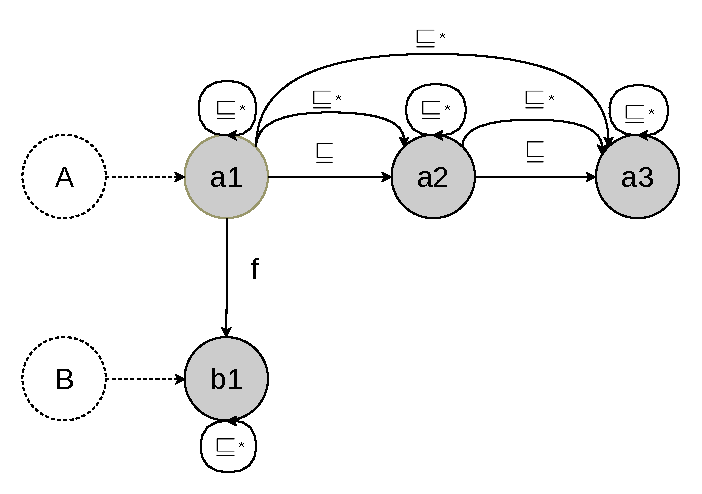
\includegraphics[scale=0.5]{extend-partial.pdf} \label{fig:extend-partial}}
\hspace{2cm}
\subfigure[] {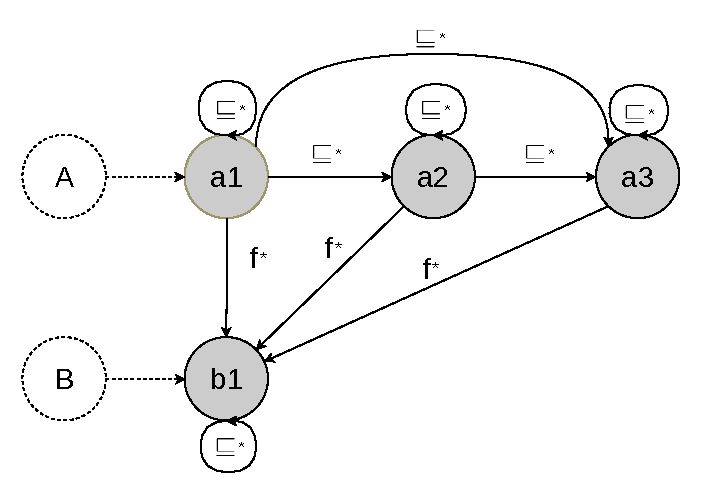
\includegraphics[scale=0.5]{extend-field-access.pdf} \label{fig:extend-field-access}}
\hspace{2cm}
\subfigure[] {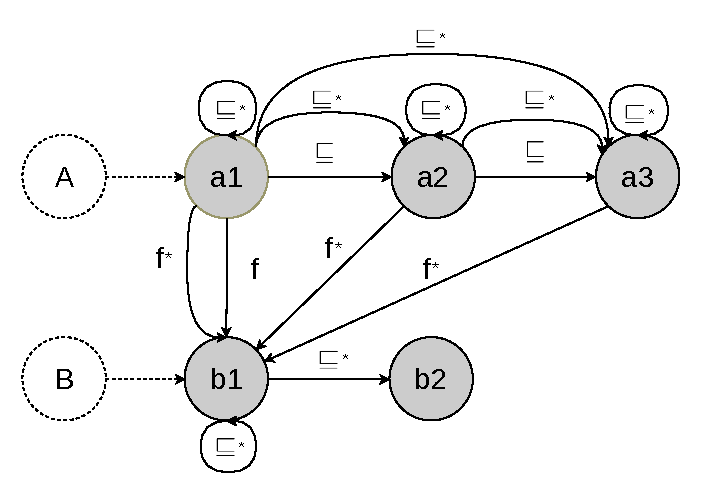
\includegraphics[scale=0.5]{extend-field-load.pdf} \label{fig:extend-field-load}}
\hspace{2cm}
\subfigure[] {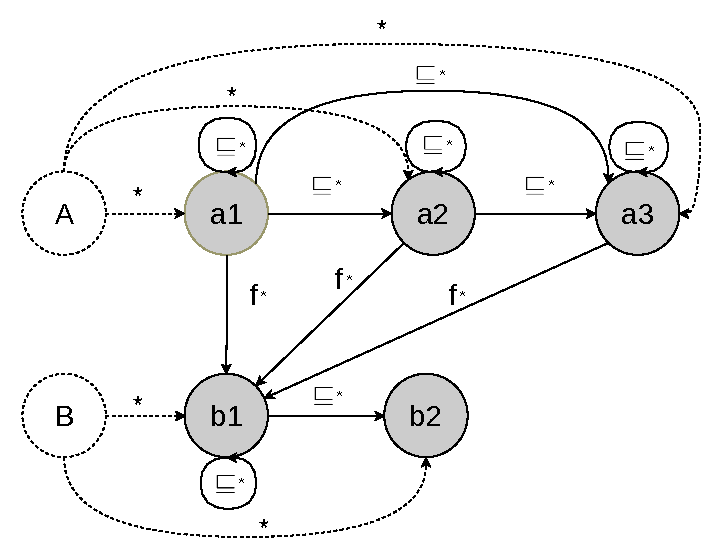
\includegraphics[scale=0.5]{extend-type-flow.pdf} \label{fig:extend-type-flow}}
\hspace{2cm}
\subfigure[] {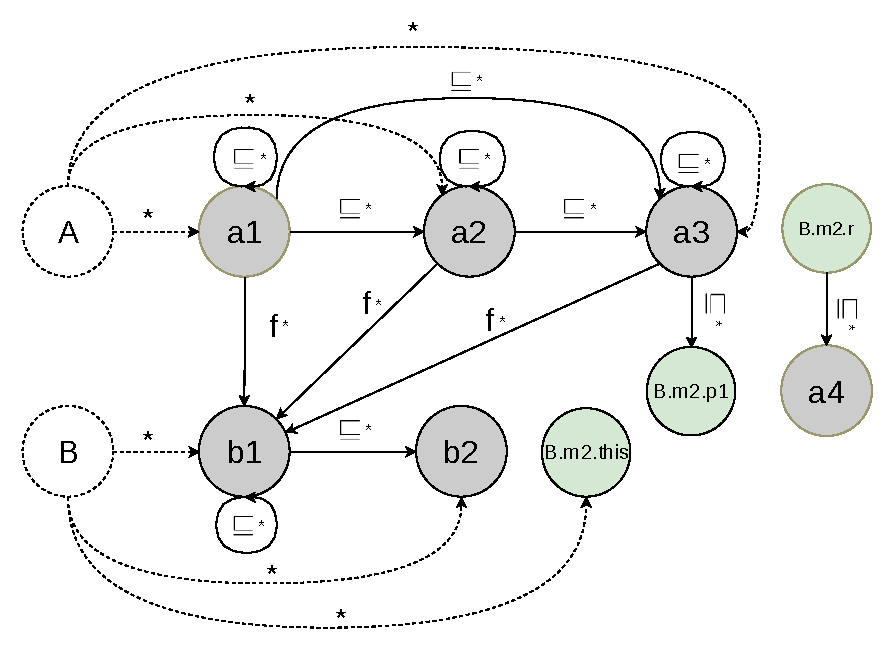
\includegraphics[scale=0.5]{extend-invocation.pdf} \label{fig:extend-invocation}}
\caption{One round of relation generation for method $m()$ in Listing~\ref{lst:relation}}
\label{fig:relations}
\end{figure}

We use five rules to extend the basic relations for  calculating a program fixpoint, which are given in the following definition 2. These rules intuitively represent propagation of type information. We put a ``$^*$'' label behind relation symbol to destinguish from basic relations.
\paragraph{Definition 2.}\label{def:extension} (Extended Relations)
\begin{enumerate}
  \item $y\less^* x$ if $x=y$ or $y\less x$ or $\exists z\in\Var:y\less^* z\wedge z\less^* x$;
  
  This rule is based on the properties of reflexive and transtive since $\less$ is a partial order relation. Besides, $y\less x$ implies $y\less^* x$. Under this rule, we extend the basic relations in~\ref{fig:basic-relation} and show the result in~\ref{fig:extend-partial}.
  
  \item $y\lhflow{f\ *}z$ if $\exists x\in\Var: x\lhflow{f}z\wedge (\exists z'\in\Var: z'\less^* y \wedge z'\less^*x)$;
  
  This rule is designed to extending field access relation. Based on the relations we generated in~\ref{fig:extend-partial}, we can generated three ``$\lhflow{f\ *}$'' relations, ``$a1 \lhflow{f\ *} b1$'', ``$a2 \lhflow{f\ *} b1$'' and ``$a3 \lhflow{f\ *} b1$'', as displayed in~\ref{fig:extend-field-access}.
  
  \item For all statements $x = y.f $, if $y\lhflow{f\ *}z$, then $z\less^* x$.

  For field load statements, only we have generated a relavant field access relation, can we extend $\less^*$ relation for target variables. \eg, From the result of~\ref{fig:extend-field-access}, we have a field access relation ``$a1\lhflow{f\ *} b1$''. So we can generate a relation ``$b1\less^* b2$'' for the field load statement ``$b2\ =\ a1.f$'' on line 7 of Listing~\ref{lst:relation}. We put the result on Fig.~\ref{fig:extend-field-load}.
  
  \item $c\tflow^* y$ if $c\tflow y$, or $\exists x\in\Var:c\tflow^* x\wedge x\less^* y$;
  
  Intuitively, this rule describe how the type information being propagated over the ``$\less^*$'' relation. We use this rule to extend the relations from~\ref{fig:extend-field-load}. The generated relations are represented in dash arrow with a label of ``$^*$'', as displayed in~\ref{fig:extend-type-flow}.
  
  \item The type information is used to resolve each method call $x = y.m(z)$.  
  \begin{equation*}
  \left.\begin{array}{l}\forall\ c\tflow^* y:\\ \forall\ m(z')\{\dots \kw{return}\ x'\}\in methods(c):\end{array}\right.\left\{\begin{array}{l}
        z\less^* c.m.z'\\
        c\tflow^* c.m.this\\
        c.m.x'\less^* x \\
        \end{array}\right.
  \end{equation*}
\end{enumerate}

These three kinds of generated relation reprensent the type flow on parameter variables, ``$this$'' reference variable and return variables, respectively.
The reaching type of variable $b2$ is $\{B\}$, \ie, we have ``$B \tflow^* b2$'', which we can extract from the result of ~\ref{fig:extend-type-flow}. That means statement ``$a4\ =\ b2.m2(a3)$'' will trigger the invocation of method $m2()$ in class $B$. In this case, we generated three relations, ``$a3 \less^* B.m2.p1$'', ``$B \tflow^* B.m2.this$'' and ``$B.m2.r \less^* a4$''. The result is shown is ~\ref{fig:extend-invocation}, where variables in method $B.m2()$ is represented as circle in green background.

We show the detail process of relation generation in one round, as displayed in~\ref{fig:relations}. In general we need more round to calculte a program fixpoint. The final relations are the least relations that satisfy constraints of Definition 2. Although the three relations are inter-dependent, one may find that without method call (i.e., Definition~\ref{def:extension}.5), a smallest model satisfying the two relations $\rightarrow^*$ (field access) and $\less^*$ (variable partial order) can be uniquely determined without considering the type flow relation $\tflow^*$.

In order to compare the precision of TFA with points-to analysis, we present a brief list of the classical subset-based points-to rules for our language in Figure~\ref{fig:constraints}, in which $\VPT$ (the var-points-to relation) maps a reference to a set of objects it may points to, and $\HPT$ (the heap-points-to relation) maps an object and a field to a set of objects. The points-to rules are mostly straightforward, except that %where
$param(type(o),m))$, $this(type(o),m))$ and $return(type(o),m)$ refer to the formal parameter, \textsf{this} reference and \textsf{return} variable of method $m$ of the class for which object $o$ is declared, respectively.

\begin{figure}%[!htbp]
	\centering %
    \begin{tabular}{|l|c|}
        \hline
    \textbf{statement} \hspace{0.5cm} & \textbf{Points-to constraints} \\
    \hline
    $x = \kwnew\ c$ & $o_i\in\VPT(x)$\\
    \hline
    $x = y $ & $\VPT(y)\subseteq\VPT(x)$\\
    \hline
    $x = y.f $ & $\forall o\in\VPT(y):\HPT(o,f)\subseteq\VPT(x)$\\
    \hline
    $x.f = y $ & $\forall o\in\VPT(x):\VPT(y)\subseteq\HPT(o,f)$\\
    \hline
    $x=y.m(z)$ &
        \(\forall o\in\VPT(y):\left\{\begin{array}{l}
        \VPT(z)\subseteq\VPT(param(type(o),m))\\
        \VPT(this(type(o),m))=\set{o}\\
        \forall x'\in return(type(o),m):\\ \hspace{35pt} \VPT(x')\subseteq\VPT(x) \end{array}\right.\)
        \\
    \hline
	\end{tabular}
\caption{Constraints for points-to analysis. \label{fig:constraints}}
\end{figure}

To this end we present the first result of the paper, which says type flow analysis has the same precision regarding type based check, such as call site resolution and cast failure check, when comparing with the points-to analysis.

\begin{Theorem}~\label{thm:tfa}
  In a context-insensitive setting, for all variables $x$ and classes $c$, $c\tflow^*x$ in TFA iff there exists an object abstraction $o$ of $c$ such that $o\in\VPT(x)$ in points-to analysis.
\end{Theorem}

\begin{proof} (sketch)
For a proof sketch, first we assume every object creation site $x = \kwnew\ c_i$ at line $i$ defines a mini-type $c_i$, and if the theorem is satisfied in this setting, a subsequent merging of mini-types into classes $c$ will preserve the result.

Moreover, we only need to prove the intraprocedural setting which is the result of Lemma 1. Because if in the intraprocedural setting the two systems have the same smallest model for all methods, then at each call site $x=y.m(a)$ both analyses will assign $y$ the same set of classes and thus resolve the call site to the same set of method definitions, and as a consequence, each method body will be given the same set of extra conditions, thus all methods will have the same initial condition for the next round iteration. Therefore, both inter-procedural systems will eventually stabilize at the same model.
\end{proof}

The following lemma focuses on the key part of the proof for Theorem~\ref{thm:tfa}, which shows that TFA and points-to analysis are equivalent regarding call site resolution locally within a function.

\paragraph{Lemma 1.}\label{lem:tfa-intra}
In a context-insensitive intraprocedural analysis where each class $c$ only syntactically appears once in the form of $\kwnew\ c$, for all variables $x$ and classes $c$, $c\tflow^*x$ iff there exists an object abstraction $o$ of type $c$ such that $o\in\VPT(x)$.
\begin{proof}
Since those constrains of the points-to analysis establish the smallest model $(\VPT, \HPT)$ with $\VPT:\Var\rightarrow\Obj$ and $\HPT:\Obj\times\Field\rightarrow\power(\Obj)$, and the three relations of type flow analysis also define the smallest model that satisfies Definition 1 and Definition~\ref{def:extension}, we prove that every model established by points-to analysis constraints is also a model of TFA, and vice versa. Then the least model of both systems must be the same, as otherwise it would lead to contradiction.

\medskip

($\star$) For the `only if' part ($\Rightarrow$), we define a function $Reaches(x)=\set{c\mid c\tflow^* x}$ which maps a variable to its reaching types in TFA, and assume a bijection $\xi:\Class\rightarrow\Obj$ that maps each class $c$ to the unique (abstract) object $o$ that is defined (and $type(o)=c$). Then we construct a function $Access:\Class\times\Field\rightarrow\power(\Class)$ and show that $(\xi(Reaches),\xi(Access))$ satisfies the points-to constraints. Define $Access(c,f)=\set{c'\mid x\lhflow{f\ *}y\wedge c\in Reaches(x)\wedge c'\in Reaches(y)}$. We prove the following cases according to the top four points-to constraints in Figure~\ref{fig:constraints}.
\begin{itemize}
\item For each statement $x = \kwnew\ c$, we have $\xi(c)\in\xi(Reaches(x))$;
\item For each statement $x = y$, we have $Reaches(y)\subseteq Reaches(x)$ and $\xi(Reaches(y))\subseteq\xi(Reaches(x))$;
\item For each statement $x.f = y$, we have $x\lhflow{f}y$, then by definition for all $c\in Reaches(x)$, and $c'\in Reaches(y)$, we have $c'\in Access(c,f)$, therefore $\xi(c')\in\xi(Reaches(y))$ we have $\xi(c')\in \xi(Access(\xi(c),f))$.
\item For each statement $x = y.f$, let $c\in Reaches(y)$, we need to show $\xi(Access(c,f))\subseteq\xi(Reaches(x))$, or equivalently, $Access(c,f)\subseteq Access(x)$. Let $c'\in Access(c,f)$, then by definition, there exist $z$, $z'$ such that $c\in Reaches(z)$, $c'\in Reaches(z')$ and $z\lhflow{f\ *}z'$. By $c\in Reaches(y)$ and Definition~\ref{def:extension}.4, we have $y\lhflow{f\ *}z'$. Then by Definition~\ref{def:extension}.1, $z'\less^*x$. Therefore $c'\in Reaches(x)$.
\end{itemize}

\medskip

($\star$) For the `if' part ($\Leftarrow$), let ($\VPT$, $\HPT$) be a model that satisfies all the top four constraints defined in Figure~\ref{fig:constraints}, and a bijection $\xi:\Class\rightarrow\Obj$, we show the following constructed relations satisfy value points-to.
\begin{itemize}
  \item For all types $c$ and variables $x$, $c\tflow^* x$ if $\xi(c)\in\VPT(x)$;
  \item For all variables $x$ and $y$, $x\less^*y$ if $\VPT(x)\subseteq\VPT(y)$;
  \item For all variables $x$ and $y$, and for all fields $f$, $x\lhflow{f\ *}y$ if for all $o_1,o_2\in\Obj$ such that $o_1\in\VPT(x)$ and $o_2\in\VPT(y)$ then $o_2\in\HPT(o_1,f)$.
\end{itemize}
We check the following cases for the three relations $\tflow^*$, $\less^*$ and $\lhflow{*}$ that are just defined from the above.
\begin{itemize}
\item For each statement $x = \kwnew\ c$, we have $\xi(c)\in\VPT(x)$, so $c\tflow^* x$ by definition.
\item For each statement $x = y$, we have $\VPT(y)\subseteq\VPT(x)$, therefore $y\less^*x$ by definition.
\item For each statement $x.f = y$, we have for all $o_1\in\VPT(x)$ and $o_2\in\VPT(y)$, $o_2\in\HPT(o_1,f)$, which derives $x\lhflow{f\ *}y$ by definition.
\item  For each statement $x = y.f$, given $y\lhflow{f\ *}z$, we need to show $z\less^* x$. Equivalently, by definition we have for all $o_1\in\VPT(y)$ and $o_2\in\VPT(z)$, $o_2\in\HPT(o_1,f)$. Since points-to relation gives $\HPT(o_1,f)\subseteq\VPT(x)$, we have $o_2\in\VPT(x)$, which derives $\VPT(z)\subseteq\VPT(x)$, the definition of $z\less^* x$.
\item The proof for the properties in the rest of Definition~\ref{def:extension} are related to transitivity of the three TFA relations, which are straightforward. We leave them for interested readers. 
\end{itemize}
\end{proof}

\section{Implementation}\label{sec:implementation}
The analysis algorithm is written in Java, and is implemented in the Soot framework, the most popular static analysis framework for Java. We use jimple as our intermediate representation. 
We do not take common types (\eg, int and float) under our consideration. That are irrelevant to our analysis. We keep method invocation from Java advanced features liked reflection or JNI as unresolvable. More detail will be discussed in \ref{subsubsec:reflection-call} and \ref{subsubsec:jni-call}. Conservative approximation is performed on invocation of methods from libraries (\eg, JDK) and array accesses. We will describe these strategies in \ref{subsubsec:library} and \ref{subsubsec:array-approximation}.

A Static analysis tool is implemented to process our algorithm and extract static result of type solution. In addition, we implement a dynamic profiler to record the run time type of variable, which can be used to compare with the static result. Detail of static analysis tool and dynamic profiler will be discuss in ~\ref{subsec:static-analysis-tool} and ~\ref{subsec:dynamic-profiler}, respectively.

\subsection{Static Analysis Tool}\label{subsec:static-analysis-tool}
Our static analysis tool is implemented in Java and aims to analyze Java programs. It takes Java bytecode files as input. Any other format of Java code will be accepted if it can be translated to jimple representation by Soot(\eg, jar files). The implementation of our static analysis tool can be splited into four step as follow.
\begin{itemize}
\item Code translation\\
Target code is loaded by Soot and translated to IR of jimple format.
\item Basic relation generation\\
We iterate all statements on jimple IR to generate those basic relations based on the basic relation difinition. 
\item Fixpoint calculation\\
After basic relations are generated, we use the extended relation rule to perform fixpoint calculation.
\item Result extraction\\
When the fixpoint is achieved, all set of reaching types of all variable are immutable. We extract those set of reaching types as our final result.
\end{itemize}
Fig~\ref{fig:static-process} shows the whole process of our static analysis tool. Data input and generated are represented in dash arrow. The final result is generated in the ``Result Extraction'' phase and represented in green background.

\begin{figure}
\centering
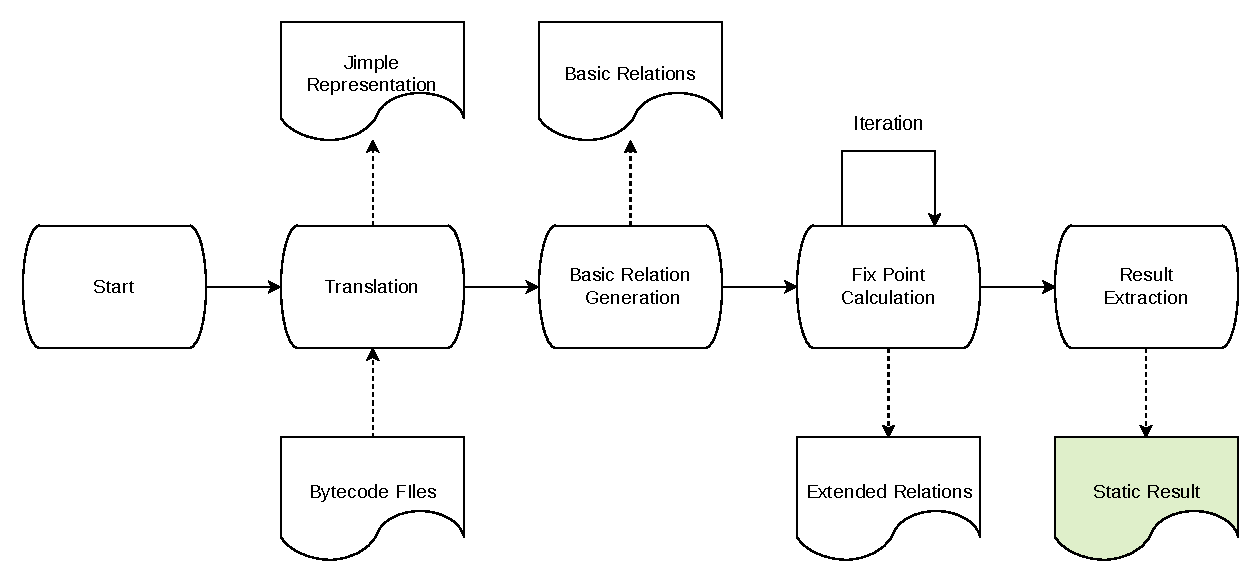
\includegraphics[width=16cm,height=6cm]{static-process.pdf}
\caption{Process of static analysis tool}
\label{fig:static-process}
\end{figure}

\subsection{Dynamic Profiler}\label{subsec:dynamic-profiler}
Since the benchmarks do not provide the grountruth of run-time type of method receiver, we implement a dynamic profiling tool to record  types which a receiver can access at run-time. To achieve this, we instrument statements into the target benchmark. After this instrumentation, the run-time type will be extracted during the benchmark execution. We consider this output as groundtruth and compare it with our static result in section ~\ref{subsec:accuracy}. There are four manners to instrument the source code to record the run-time type of a method receiver.
\begin{itemize}
\item Insert First\\
In this manner, the type-recorded statements will be insert before the first statement of a method block and the type of ``this'' reference in that method will be recorded. The reason we only have to record ``this'' reference is that a receiver is always passed into ``this'' reference in a method, except for static methods. 
\item Insert Before\\
Statements will be inserted before invocations and the type of receiver will be recorded in this manner. It is more straightforward than the method we discuss about recording ``this'' reference.
\item Insert Last\\
This manner is similar with ``Insert First'', except that statements are inserted after the last statement of a method block. We also record ``this'' reference in this way.
\item Insert After\\
Statments will be inserted right after invocations and the type of receiver will be recorded. It is similar with ``Insert Before'', except that statements are inserted at different position. We take this manner in our implementation and the reason will be discuss in section ~\ref{subsubsec:instrument}
\end{itemize}
%\subsubsection{Insert First}\label{subsubsec:insert-first}
%In this manner, the type-recorded statements will be insert before the first statement of a method block and the type of ``this'' reference in that method will be recorded. The reason we only have to record ``this'' reference is that a receiver is always passed into ``this'' reference in a method, except for static methods. 
%\subsubsection{Insert Before}\label{subsubsec:insert-before}
%Statements will be inserted before invocations and the type of receiver will be recorded in this manner. It is more straightforward than the method we discuss about recording ``this'' reference.
%\subsubsection{Insert Last}\label{subsubsec:insert-last}
%This manner is similar with ``Insert First'', except that statements are inserted after the last statement of a method block. We also record ``this'' reference in this way.
%\subsubsection{Insert After}\label{subsubsec:insert-after}
%Statments will be inserted right after invocations and the type of receiver will be recorded. It is similar with ``Insert Before'', except that statements are inserted at different position. We take this manner in our implementation and the reason will be discuss in section ~\ref{subsubsec:instrument}
\subsubsection{Our Instrumentation Manner}\label{subsubsec:instrument}
We take ``Insert After'' as our instrumentation manner. The reason is mainly due to the Java specification of constructor that the first statement in constructor should be either another constructor of its own or its super class. Therefore, we will get JVM voilation error if we instrument a statement before the first statement in construtor. We illustrate this example on Listing~\ref{lst:spec-constructor}. So both ``Insert First'' and ``Insert Before'' manners can not be applied under this circumstance. We choose ``Insert After'' over ``Insert Last'' for reason that it's more straightforward. The code before and after instrumentation are shown in Listing~\ref{lst:before-instru} and Listing~\ref{lst:after-instru}, respectively. For Listing~\ref{lst:after-instru}, at line 5, the funtion $RecordUtils.id()$ takes an invocation expression ($invokeExprssion$) and a method receiver ($b$) as parameters and return an unique representation string for this invocation. For this example, the unique representation is ``A:m1:b:B:m2:4''. This means $b$ will call method $m2$ of class $B$, at line 4 in method $m1$ of class $A$. It also shows that $b$ is of type $B$ at this position.

\begin{lstlisting}[caption={Java specification on constructor},label={lst:spec-constructor}]
class A {
  public A() {
    //insert statements here will violate JVM specification
    super();	//invoke super class constructor
  }
  public A(int i) {
    //insert statements here will violate JVM specification
    this();    //inovke another constructor of its own
  }
}
\end{lstlisting}

\begin{lstlisting}[caption={Example code before instrumentation},label={lst:before-instru}]
class A {
  public void m1() {
    B b = new B();
    b.m2();    //invocation here
  }
}
\end{lstlisting}

\begin{lstlisting}[caption={Example code after instrumentation},label={lst:after-instru}]
class A {
  public void m1() {
    B b = new B();
    b.m2();    //invocation here
    String record = RecordUtils.id(invokeExpression, b);
    RecordUtils.record(record);
  }
}
\end{lstlisting}

\section{Evaluation}\label{sec:evaluation}
We evaluate our approach by measuring its performance on SPECjvm2008, which contains $12$ benchmark programs in total. We conduct all of our experiments on a laptop equipped with an Intel i5-8250U CPU at 1.60 GHz and 8 GB memory, running Ubuntu 16.04LTS with OpenJDK 1.8.0.

We compare our approach against the default implementation of Class Hierarchy Analysis (CHA) and context-insensitive points-to analysis that are implemented by Soot team. The reason we do not compare against Variable Type Analysis (VTA) due to its unavaliable implementation. The only avaliable implementation for Java is also implemented by Soot team, but it is embeded as a subprocess to optimize points-to analysis. Under this circumstance, we compare our approach against VTA in precision with manual analysis in section~\ref{sec:introduction}. Implementation of VTA will be left for our future work. The choice of the context-insensitive points-to analysis is due to our approach also being context-insensitive, thus the results will be comparable. We use iteration algorithm for points-to analysis to calculate a fixpoint for the same reason. In the following tables we use CHA, PTA and TFA to refer to the results related to class hierarchy analysis, points-to analysis and type flow analysis, respectively. During the evaluation the following tow research questions are addressed.
\begin{itemize}
\item \textbf{RQ1} How efficient is our approach compared with the traditional class hierarchy analysis and points-to analysis?
\item \textbf{RQ2} How accurate is our algorithm when comparing with the other analysis?
\end{itemize}
We answer these two questions in section~\ref{subsec:efficiency} and section~\ref{subsec:accuracy}, respetively.

\subsection{Efficiency}\label{subsec:efficiency}
We executed each benchmark program $10$ times with the CHA, PTA and TFA algorithms. We calculated the average time consumption (in seconds) as displayed at column \textbf{T$_{CHA}$}(s), \textbf{T$_{PTA}$}(s) and \textbf{T$_{TFA}$}(s) of the Table in Fig.~\ref{fig:TimeCost}. We counted the sizes of each generated realtion (\ie, the type flow realtion `$\tflow$', variable partial order `$\less$' and the field access relation `$\hflow$'). It provides an estimation of size for the problem we are treating. The result shows that our approach consums more time than CHA, for the reason that CHA do not have to analyze detail logic inside the program but only analyze the class and interface hierarchical structure. TFA is in general more efficient than points-to analysis. The runtime cost in TFA basically depends on the size of generated relations, as well as the relational complexity as most of the time is consumed to calculate a fixpoint. For PTA it also require extra time for maintaining and updating a heap abstraction.

\begin{figure}\centering
\begin{threeparttable}[b]
%\begin{table}[!htbp]\centering
\begin{tabular}{lccccccc}
	\fullhline
	\textbf{Benchmark} & \hspace{5pt}\textbf{T$_{\textsf{CHA}}(s)$}& \hspace{5pt}\textbf{T$_{\textsf{PTA}}(s)$} & \hspace{5pt}\textbf{T$_{\textsf{TFA}}(s)$} & \hspace{5pt}\textbf{R${\tflow}$}\hspace{5pt} & \hspace{5pt}\textbf{R$_{\less}$}\hspace{5pt} & \hspace{5pt}\textbf{R${\rightarrow}$} &\hspace{5pt}\textbf{R$_{total}$}\hspace{2pt}\\
	\fullhline
check & 5.33 & 71.98 & 10.46 & 6847 & 15599 & 10089 & 32535\\
compiler & 5.76 & 72.01 & 11.48 & 6665 & 14898 & 10433 & 31996\\
compress & 5.72 & 71.06 & 12.19 & 6410 & 14344 & 10322 & 31076\\
crypto & 5.60 & 69.25 & 9.21 & 6459 & 14424 & 10152 & 31035\\
derby & 5.83 & 70.57 & 11.65 & 6887 & 14853 & 10603 & 32343\\
helloworld & 6.26 & 70.72 & 13.10 & 6149 & 13652 & 10071 & 29872\\
mpegaudio & 6.29 & 70.45 & 10.65 & 6197 & 13737 & 10084 & 30018\\
scimark & 6.77 & 71.37 & 11.24 & 6366 & 14678 & 10214 & 31258\\
serial & 7.06 & 70.41 & 10.98 & 6627 & 14309 & 10341 & 31277\\
startup & 5.62 & 69.09 & 10.73 & 6239 & 13723 & 10094 & 30056\\
sunflow & 5.58 & 72.93 & 11.12 & 6167 & 13675 & 10077 & 29919\\
xml & 6.55 & 139.08 & 13.84 & 6866 & 16039 & 11060 & 33965\\
	\fullhline
\end{tabular}
\caption{Runtime cost with different analysis}
\label{fig:TimeCost}
\begin{tablenotes}
  \item[1] \textbf{R}$_{relation}$ denotes different type of relation we generated.
\end{tablenotes}
%\end{table}
\end{threeparttable}
\end{figure}

\subsection{Accuracy}\label{subsec:accuracy}
We answer the seconde question about accuracy in two indexes: precision and recall. Their difinitions are given in equation 1 and 2, respectively.
\begin{equation}
precision =  \dfrac{M}{S} 
\end{equation}
\begin{equation}
recall = \dfrac{M}{D} 
\end{equation}
``D'' stands for the number of dynamic record, ``S'' refers to the numer of static record, and ``M'' represents the number of matching record. 

A sound algorithm should catch all type information in run time, \ie, the recall should be $100\%$. Precision indicates how accurate the generated set of types is. In general, a more acurrate algorithm often generate a smaller set of types for each calling variable. We calculate recall and precision of different approach, as displayed in Fig.~\ref{fig:accuracy}

The result shows that in general our approach can achieve higher precision than CHA and closer precision than PTA. The imprecision is mainly due to our approximation on library invocation and array, which we will discuss in section~\ref{subsubsec:library} and section~\ref{subsubsec:array-approximation}. Besides, the code coverage will issue imprecision since SPECjvm provides common codes for all benchmarks and some of them would not be excuted when a specific benchmark is excuting, \ie, these codes will be analyzed statically but not generate any record in run time.

For soundness, the recall of both TFA and PTA can not achieve to $1.00$ in most benchmarks except $helloworld$. We analyzed those missed records and find out the reason is due to some Java advance features, liked reflection call and JNI call, which we will describe in section~\ref{subsubsec:reflection-call} and section~\ref{subsubsec:jni-call}. In addition,  callback mechanism will raise unsoundness under our treatment on reflection, JNI and library call. We will discuss it in section~\ref{subsubsec:callback}. The result shows that PTA produces lower recall than TFA in general. We study the reason for this gap from read the source code of Soot and find out it is due to the on-the-fly reachability analysis used on PTA implemented by Soot team. Method invoked by reflection, or invoked as a callback function inside reflection, JNI and library, will be denoted as unreachable under this analysis. As a consequence, some methods would not be analyzed by PTA. Note that even the unreachable method would not be analyzed, a variable receiving its type from JDK would be assigned to possible types based on the preprocessing from Soot. Such that the set of possible reaching types for these variables would not be empty.
\begin{figure}\centering
%\begin{table}[!htbp]\centering
\begin{threeparttable}[b]
\begin{tabular}{lcccccccccc}
	\fullhline
	\textbf{Benchmark} & \textbf{D} & \textbf{M$_{CHA}$} & \textbf{M$_{PTA}$} & \textbf{M$_{TFA}$} & \textbf{R$_{CHA}$} & \textbf{R$_{PTA}$} & \textbf{R$_{TFA}$} & \textbf{P$_{CHA}$} & \textbf{P$_{PTA}$} & \textbf{P$_{TFA}$} \hspace{2pt}\\
	\fullhline
check & 150 & 150 & 145 & 145 & 1.00 & 0.97 & 0.97 & 0.07 & 0.19 & 0.18\\
compiler & 515 & 515 & 463 & 506 & 1.00 & 0.90 & 0.98 & 0.28 & 0.81 & 0.70\\
compress & 353 & 353 & 330 & 345 & 1.00 & 0.93 & 0.98 & 0.19 & 0.49 & 0.46\\
crypto & 454 & 454 & 393 & 407 & 1.00 & 0.87 & 0.90 & 0.25 & 0.70 & 0.65\\
derby & 639 & 639 & 603 & 632 & 1.00 & 0.94 & 0.99 & 0.35 & 0.97 & 0.88\\
helloworld & 21 & 21 & 21 & 21 & 1.00 & 1.00 & 1.00 & 0.01 & 0.03 & 0.03\\
mpegaudio & 255 & 255 & 241 & 248 & 1.00 & 0.95 & 0.97 & 0.15 & 0.40 & 0.37\\
scimark & 386 & 386 & 357 & 362 & 1.00 & 0.92 & 0.94 & 0.20 & 0.54 & 0.50\\
serial & 458 & 458 & 354 & 410 & 1.00 & 0.77 & 0.90 & 0.18 & 0.67 & 0.62\\
startup & 1429 & 1429 & 1358 & 1360 & 1.00 & 0.95 & 0.95 & 0.82 & 2.23 & 2.07\\
sunflow & 226 & 226 & 208 & 217 & 1.00 & 0.92 & 0.96 & 0.13 & 0.36 & 0.33\\
xml & 521 & 521 & 436 & 504 & 1.00 & 0.84 & 0.97 & 0.27 & 0.81 & 0.65\\
	\fullhline
\end{tabular}
\caption{Accuracy with different analysis}
\label{fig:accuracy}
\begin{tablenotes}
  \item[1] \textbf{D} denotes dynamic records.
  \item[2] \textbf{M$_{algorithm}$}, \textbf{R$_{algorithm}$}, \textbf{P$_{algorithm}$} denote matching count, recall and precision of different algorithms, respectively.
\end{tablenotes}
\end{threeparttable}
%\end{table}
\end{figure}

\subsubsection{Reflection Call}\label{subsubsec:reflection-call}
Reflection in Java programming language is a advanced feature which provides ability to inspect and manipulate a Java class at runtime. It brings in extra complexity on programs and the behaviour is hard to predict statically. In Listing~\ref{lst:reflection} we pick some codes using reflection in the benchmark programs to discuss how reflection works and what is our treatment on that. Note that we reorganize and simplify the real code a little to concentrate on the main point of reflection usage. We discuss in three cases:
\begin{itemize}
\item Object Creation \\
Related codes range from line 6 to 10. A new obejct of type ``SPECJVMBenchmarkBase'' will be created by invoking the method ``$newInstance()$'' on variable $c$ at line 10. $c$ is an object of ``Constructor'' type and it refers to a specific constructor of class ``SPECJVMBenchmarkBase''. Our method discard the type information of new object in these case because it's difficult to statically identify which constructor will be invoked. \eg, At line 6, If statement $Class.forName()$ receive argument from outside liked user input or loading file with content of class name, then we could not find out the real type of $benchmarkClass$. As a result, the run time type of $c$ and $benchmark$ could not be identified neither.
\item Method Invocation\\
After a new object is instantiated, we can get an object of ``Method'' type, referring to a specific method of a class, and call the method named ``invoke()'' of that object. This effect is just like a normal invocation at line 12. The invocation receiver is passed to the first argument of method ``invoke()''. If this invocation is static, a \textbf{null} reference will be passed to the first argument. We do not consider these effects of method invocation in reflection manner for the same reason we discuss about object creation.
\item Field Modification\\
The way to change a field using reflection is similar to processing method invocation. The last two line illustrate changing value of a field named ``f'' on object ``benchmark'' into a new object. We discard this effect as well because of the difficulty on analyzing which class holds the target field.
\end{itemize}
\begin{lstlisting}[caption={Example code of reflection},label={lst:reflection}]
public static void runSimple(Class benchmarkClass, String [] args) {
  ...
  ...
  Class[] cArgs = { BenchmarkResult.class, int.class };
  Object[] inArgs = { bmResult, Integer.valueOf(1)};
  Class benchmarkClass = Class.forName("spec.harness.SpecJVMBenchmarkBase");
  Constructor c = benchmarkClass.getConstructor(cArgs);

  // Object creation using reflection
  SpecJVMBenchmarkBase benchmark = (SpecJVMBenchmarkBase)c.newInstance(inArgs);
  // normal method invocation
  benchmark.harnessMain();
  
  // method invocation
  Method harnessMain = benchmarkClass.getMethod("harnessMain", new Class[]{});
  // just like line 11 but in reflection manner
  harnessMain.invoke(benchmark, new Object[]{}); 
  
  Method setup = benchmarkClass.getMethod( "setupBenchmark", new Class[]{});
  // static invocation
  setup.invoke(null, new Object[]{});
  
  // field modification
  Field f = benchmarkClass.getField("f");
  f.set(benchmark, new Object());
}
\end{lstlisting}

\subsubsection{Java Native Interface Call}\label{subsubsec:jni-call}
Java Native Interface (JNI) is a standard Java programming interface which provide ability for Java code to interoperate with application or library written in other programming languages, such as C, C++ or assembly. We show the usage of JNI in Listing~\ref{lst:jni}. Method ``$m()$'' is defined as a native method and should not be implemented in Java. This program will load a native library named ``$lib$'', in which the method ``$m()$'' is actually implemented in different program languages. We do not consider JNI calls in our algorithm since the code is not written in Java. Analyzing that code and the communication between Java and other languages are out of our research scope. As a consequence, the effect of that invocation ``$a.m()$'' at line 8 will be discarded.

\begin{lstlisting}[caption={Example code of JNI},label={lst:jni}]
public class A {
  public native void m();
  static {
    System.loadLibrary("lib");
  }
  public static void main(String[] args) {
    A a = new A();
    a.m(); <---
  }
}
\end{lstlisting}

\subsubsection{Library}\label{subsubsec:library}
Library are those codes included in the application and used to accomplish specific function(\eg, JDK library, three-party library). Listing~\ref{lst:jdk} shows a common case of JDK invocation. We do not analyze the detail logic inside library code which are written at line 10-11. Instead, we perform an over approximation on library invocation, based on the method difinition which appears at line 9. We assume that library invocation will return the difinition type and any subtype of this difinition type as the result type. For Listing~\ref{lst:jdk}, $sb2$ will receive $\{StringBuilder,\ any\_subtype\_of\_StringBuilder\}$ as the set of reaching types under this over approximation strategy.

\begin{lstlisting}[caption={Example of JDK library call},label={lst:jdk}]
import java.lang.StringBuilder;

public void m() {
  StringBuilder sb = new StringBuilder();
  StringBuilder sb2 = sb.append("abc"); <---
}

//  @Override
//  public StringBuilder append(String str) {
//    ...
//    ...
//  }
\end{lstlisting}

\subsubsection{Array Approximation}\label{subsubsec:array-approximation}
We perform a conservative treatment on array accesses that all type information that flows to one member of an array flows to all members of that array. Codes in Listing~\ref{lst:array} are used to explain how this approximation works. Type information of $A$ and $B$ are flow to the first member and the second member of array $arr$, respectively. We approximate that these two type information flow to array $arr$. Loadding an element of array will receive all types that array can access(\eg, $b$ will receive $\{A, B\}$ as the set of reaching types, which is the same set of types that array $arr$ can access).

\begin{lstlisting}[caption={Example of array access},label={lst:array}]
public void m() {
	Object[] arr = new Object[2]{};
	arr[1] = new A();
	arr[2] = new B();
	Object b = arr[1];  <---
}
\end{lstlisting}

\subsubsection{Callback}\label{subsubsec:callback}
A callback function is known as a ``call-after'' function. It is widely used in programs. By passing a argument to one invocation as the receiver which is expected to trigger a callback invocation. In functional language a callback funtion can be passed as argument directly. Listing~\ref{lst:callback}
 shows the callback mechanism. The function $callback()$ will be invoked after the invocation of $trigger()$. Since we do not analyze the effect of reflection call, JNI call, and library call, we are unable to catch the type flow information inside $a.trigger(b)$ if it happens to be one of these calls (\eg, $trigger()$ is a method of a library class). Note that we only conservatively approximate on the return type of a library invocation, but not analyze the detail logic inside a library method.
\begin{lstlisting}[caption={Callback mechanism},label={lst:callback}]
class A {
	public void trigger(B b) {
		b.callback();  // here the callback function actually executes
	}
}

class B {
	public void callback() {...}
	public void static main() {
		A a = new A();
		B b = new B();
		a.trigger(b);
 	}
}
\end{lstlisting}

\section{Related Work}\label{sec:related-work}
There are not many works focusing on general purpose call graph construction algorithms, and we give a brief review of these works first.

As stated in the introduction, Class Hierarchy Analysis (CHA)~\cite{Dean1995,Fernandez1995}, Rapid Type Analysis (RTA)~\cite{Bacon1996} and Variable Type Analysis (VTA)~\cite{Sundaresan2000} are efficient algorithms that conservatively resolves call sites without any help from points-to analysis. Grove et al.~\cite{Grove1997} introduced an approach to model context-sensitive and context-insensitive call graph construction. They define call graph in terms of three algorithm-specific parameter partial orders, and provide a method called Monotonic Refinement, potentially adding to the class sets of local variables and adding new contours to call sites, load sites, and store sites.
%
Tip and Palsberg~\cite{Tip2000} Proposed four propagation-based call graph construction algorithms, CTA, MTA, FTA and XTA. CTA uses distinct sets for classes, MTA uses distinct sets for classes and fields, FTA uses distinct sets for classes and methods, and XTA uses distinct
sets for classes, fields, and methods. The constructed call graphs tend to contain slightly fewer method definitions when compared to RTA. It has been shown that associating a distinct set of types with each method in a class has a significantly greater impact on precision than using a distinct set for each field in a class. Reif et al.~\cite{Reif2016} study the construction of call graphs for Java libraries that abstract over all potential library usages, in a so-called \emph{open world} approach. They invented two concrete call graph algorithms for libraries based on adaptations of the CHA algorithm, to be used for software quality and security issues. In general they are interested in analyzing library without knowing client application, which is complementary to our work that has focus on client program while treating library calls as end nodes.

Call graphs may serve as a basis for points-to analysis, but often a points-to analysis implicitly computes a call graph on-the-fly, such as the context insensitive points-to algorithm implemented in Soot using SPARK~\cite{Lhotak2003}. Most context-sensitive points-to analysis algorithms (e.g.,~\cite{Milanova2005,Sridharan2006,Smaragdakis11,Tan16}) progress call edges together with value flow, to our knowledge. The main distinction of our approach from these points-to analysis is the usage of an abstract heap, as we are only interested in the actual reaching types of the receiver of a call. Nevertheless, unlike CHA and VTA, our methodology can be extended to context-sensitive~settings.

Regarding the treatment of flow analysis in our algorithm, downcast analysis has been studied in region inference which is a special memory management scheme for preventing dangling pointers or improving precision in garbage collection in object-oriented programming languages~\cite{Boyapati2003,Chin2004}.  These works are type-based analysis, while our methodology belongs to traditional static program analysis. Similar ideas regarding value flow can also be found in the graph-reachability based formulation (e.g.~\cite{Reps1997,Lu2013}) to which all distributed data flow analyses can be adopted.

\section{Conclusion}\label{sec:conclusion}
In this paper we have proposed Type Flow Analysis (TFA), an algorithm that constructs call graph edges for Object-Oriented programming languages.

\label{lastpage}


\end{document}
